\documentclass[
	% Basic information
	StudentName     = 姓名,
	StudentID       = 学号,
	AdvisorName     = 指导教师,
	Grade           = 年级,
	Major           = 专业,
	Department      = 一个很长很长的名字,
	% Submit time
	SubmitYear		= 2022,
	SubmitMonth		= 5,
	% Title
	Title           = 论文中文题目,
	TitleEng        = {{English Title}}
]{cauc_thesis}


% 导入页面命令
\newcommand{\inputpage}[1]{
	\input{settings/#1}
}



\begin{document}
	\inputpage{cover}
	
	%%%% 摘要
	\newpage
	\setcounter{page}{1}
	\pagenumbering{Roman}
	\setlength{\headsep}{1.224cm}
	\begin{center}
		\zihao{3}\fakehei 摘\quad 要
	\end{center}
	\vspace{21pt}
	\zihao{-4}
	
	
	\setlength{\baselineskip}{20pt}
	% ---------------摘要----------------------
	摘要应具有独立性和自含性,即不需阅读报告、论文的全文,就能获得必要的信息,供读者确定有无必要阅读全文。摘要是一篇完整的短文,一般应说明研究工作目的、实验方法、结果和最终结论等,而重点是结果和结论。
	
	摘要要求结构严谨,表达简明,语义确切,字数300-500字为宜。
	
	摘要中应排除本学科领域已成为常识的内容;不要把应在文献综述中出现的内容写入摘要;也不要对论文内容作诠释和评论(尤其是自我评价)。
	
	用第三人称,不必使用"本文"、"作者"等作为主语。
	
	单位制一律换算成国际标准计量单位制,除了实在无法变通以外,一般不用数学公式和化学结构式,不得出现插图、表格。
	
	缩略语、简称、代号,除了相邻专业的读者也能清楚理解的以外,在首次出现时必须加以说明。
	\newline
	\newline
	\indent\zihao{-4}{\bf 关键词:}\zihao{-4} 关键词1;关键词2;关键词3;关键词4

	%%%% 
	\newpage
	\setlength{\headsep}{1.224cm}
	\begin{center}
		\zihao{3} \textbf{Abstract} 
	\end{center}
	\vspace{21pt}
	\zihao{-4}
	% ------------------Abstract--------------------------
	英文摘要另起一页,内容应与"中文摘要"对应。使用第三人称,用现在时态编写。
	\newline
	\newline
	\indent\zihao{-4}\textbf{Key Words: }\zihao{-4}\songti Keyword1; Keyword2; Keyword3; Keyword4;
	
	%%%% 目录
	\newpage
	\setlength{\headsep}{-0.3cm}
	% 去除页码
	\pagenumbering{gobble}
	\tableofcontents
	\clearpage	% 去除页码命令终止
	\setcounter{page}{1}
	\pagenumbering{arabic}

	
	\setlength{\headsep}{0.624cm}
	\fancypagestyle{plain}{
		\pagestyle{fancy}
	}%在章节页也显示页眉
	% **********绪论**************
	\pagestyle{fancy}
	\setlength{\baselineskip}{20pt}
	{\centering\chapter{绪论}}
	\setlength{\baselineskip}{20pt}
	一篇完整的毕业设计或论文 \cite{reflabel1,reflabel2} 通常由题目、摘要、目录、正文、结论、参考文献、致谢、附录等几部分构成,除外语类专业外一律采用汉语撰写。
	
	
	本科毕业设计论文的总篇\cite{reflabel3,reflabel4,reflabel5}幅包括图表在内(附录除外),理科类一般8000字以上,工科、文科类以1-1.5万字为宜,最多不要超过2万字。
	
	\section{题目}
	
	题目应该简短、明确,要有概括性。让人看后能大致了解文章的确切内容、专业特点和学科范畴。因此要明确、准确、精炼地直接概括描述所研究的主要内容和方法,题目字数要适当,一般不宜超过20字。如果有些细节必须放进题目里,为避免冗长,可以将细节放进副标题中。
	
	\section{摘要}
	
	摘要在毕业设计说明书或论文的主体之前,用中英文撰写,要求参见中、英文摘要说明。
	
	\section{目录}
	
	显示标题级别最多3级并标明页号。注意目录内容应与正文中的标题相一致,页码相对应。
	
	\section{正文}
	
	正文第1章为绪论,说明研究工作的目的、意义及应用领域;国内外相关领域的研究及应用现状,存在的缺陷或不足;拟采用的方法及研究内容;拟解决的关键技术问题和预期成果等。应言简意赅,不要与摘要雷同,更不要成为摘要的注释。一般教科书中有的知识,在引言中不必赘述。
	
	正文的主体是对研究工作的详细表述,可以分章论述。其内容包括:研究工作的基本前提、假设和条件;模型的建立,实验方案的拟定;设计计算的主要方法和内容;实验方法、内容及其分析;理论论证在课题中的应用,课题得出的结果,以及对结果的讨论等。
	
	理论模型建立及分析、系统设计及分析应完善、合理;试验验证方法、过程及结论应充分验证所建立的理论模型或所设计的系统的正确性,对可能出现的问题或不足应进行深入分析。
	
	如有必要论文中还应加入本研究的经济特性的分析,如投资效率、利润情况、对环境污染情况的讨论等。
	
	\section{结论}
	
	结论是整篇论文的归结,对全篇论文起到画龙点睛的作用,必须单独书写。结论的内容不只是前面实验结果部分已经得出的研究结果的简单重复,应对论文研究中存在的不足及需要进一步改进或完善的内容进行适当地阐述。
	
	\section{参考文献}
	
	参考文献只列出作者直接阅读过、在正文中被引用过的文献资料。参考文献一律放在论文结束后,按文中引用的顺序一一列出。
	
	参考文献8-15篇,包括近五年的科技论文和至少2篇的外文资料。
	\section{致谢}
	
	限一页。对帮助过自己的人表达谢意不仅是一种礼貌,更是对他人劳动的尊重,是治学者应有的思想作风,但也应避免过于浮夸。
	
	\section{附录(或调研报告)}
	
	附录不是必须,内容一般包括正文内不便列出的冗长公式推导、辅助性数学工具、符号说明(含缩写)、计算程序及说明等,也可以是调研报告。
	
	附录的内容应有独立的完整性,并应有标题以概括附录的内容。多个附录要按顺序编号,在正文中提到有关内容时要注明参看附录。
	
	{\centering\chapter{正文要求}}
	
	本科生毕业设计(论文)的正文是主体部分,要着重反映自己的工作,突出新的见解,例如新思想、新观点、新规律、新研究方法、新结果等。正文可以包括:调查对象、实验和观测方法、仪器设备、材料原料、实验和观测结果、计算方法和编程原理、数据资料、经过加工整理的图表、形成的论点和导出的结论等。
	
	正文要求论点正确,推理严数据可靠,文字精练,条理分明,文字图表清晰整齐。利用别人研究成果必须附加说明。引用前人材料必须引证原著文字。在论文的行文上,要注意语句通顺,达到科技论文所必须具备的"正确、准确、明确"的要求。
	
	由于研究工作涉及的学科、选题、研究方法、工作进程、结果表达方式等有很大的差异,不对正文内容作统一硬性的规定。但是,必须实事求是,合乎逻辑,层次分明。
	
	\section{格式要求}
	\subsection{页面设置及格式}
	
	字体:论文中出现的英文字母及数字均设置为小四号{\rm Times New Roman}
	
	纸型:A4(ISO)纸,单面打印。
	
	页边距:上2.5cm,下2.5cm,左3cm,右2.5cm。
	
	页眉:1.5cm,显示"中国民航大学本科毕业设计论文",采用五号宋体、居中,从正文第一页起始。
	
	页脚:1.75cm,页码为阿拉伯数字,五号宋体,居中,正文起始页码为1(阿拉伯数字)。
	
	装订线:0cm,左侧装订。
	
	封面:采用我校统一格式。
	
	摘要:"摘要"二字为三号黑体,居中,行间距20磅,段前18磅,段后30磅,两字间空两个中文字符;摘要内容为小四号宋体。英文摘要"Abstract"为三号Times New Roman,居中,行间距20磅,段前18磅,段后30磅;内容为小四号Times New Roman。
	
	关键词:关键词要与上文空一行,"关键词"三字为小四号宋体加粗,紧随其后为关键词,采用小四号宋体。"Key
	words"一词为小四号Times New Roman加粗,紧随其后为关键词,用小四号Times New Roman。
	
	目录:"目录"二字为三号黑体,居中,行间距20磅,段前18磅,段后30磅,两字间空两个中文字符。一级标题采用小四黑体,其余采用小四号宋体。页码放在行末,目录内容和页码之间用虚线连接。低级标题比高级标题缩进两个中文字符。
	
	正文:中文为小四号宋体,英文字母及数字为小四号Times New Roman,段落行间距为20磅,段前段后均为0。首行缩进2个中文字符。
	
	参考文献:"参考文献"四字采用一级标题,内容的字体为小四宋体。参考文献在文内的标注采用顺序编码制,对引用的文献,按它们在论文中出现的先后用阿拉伯数字连续编码,将序号置于上标方括号内,如"……对此做了研究[3]"。注意只有文献第一次在文中出现时才编序号,即一篇文献只有一个序号,若某文献在文中被多次引用,在几个引用处都要标注同一个序号。若在正文的一处引用了多篇文献,标注时只用一个方括号,括号内列写这几篇文献的序号:若几个序号是连续的,只标注起、止序号,两序号之间加半字线"-"号;若几个序号不连续,各序号之间加逗号,如“[3-5, 8]”表示在该处引用了3、4、5和8号文献。
	
	致谢:"致谢"用一级标题两字中间空两个中文字符,顶格书写,行间距20磅,段前18磅,段后30磅。致谢内容为小四号宋体。
	
	附录:"附录:"及其标题用一级标题,居中,行间距20磅,段前18磅,段后30磅。内容的字体为小四宋体。附录中的图表公式另编排序号,与正文分开。
	
	\subsection{标题要求}
	
	标题要重点突出,层次要清楚,简明扼要。章节编号方法采用分级阿拉伯数字编号方法,即"1"、"2.1"、"3.2.1"等,两级之间用下角圆点隔开,各层标题均单独占行书写,每一级的末尾不加标点。
	
	第一级标题要另起一页,用三号黑体居中,行间距20磅,段前18磅,段后30磅,数字与标题之间空两格;
	
	第二级标题为四号黑体,行间距20磅,段前0.5行,段后0.5行,序数顶格书写,数字与标题之间空两格;
	
	第三级标题为小四号黑体,行间距20磅,段前0.5行,段后0.5行,序数顶格书写,数字与标题之间空两格。
	
	\subsection{标题设置方法}
	
	1.选中设置为标题的字行。
	
	2.点击左上角的样式栏,选择标题级别。一级标题为标题1,二级标题为标题2,三级标题为标题3。
	
	3.按要求进行格式调整,如字体、对齐方式、字号等。
	
	4.所有标题设置完毕后,将光标移至目录页上,点击"插入"、"引用"、"索引和目录",插入目录并按要求调整格式。如果已插入目录,修改时要用右键点击目录,选择"更新域",然后选择"更新整个目录"并按要求调整格式。
	
	\subsection{页眉设置方法}
	
	点击"视图"、"页眉和页脚",设置页眉为"中国民航大学本科毕业设计论文",字体为宋体五号,居中。
	
	\section{语言表述}
	
	\subsection{语言表述}
	1.正文应层次分明、数据可靠、推理严谨、立论正确。论述必须简明扼要、重点突出,对同行专业人员已熟知的常识内容,尽量减少叙述。
	
	2.正文应采用普通话,用词准确,语法正确、符合逻辑,文句力求精炼简明、深入浅出、通顺易懂。避免采用口语俚语、生涩词语以及非学术、专业术语。
	
	3.正文中如出现一些非通用性的新名词、新术语或新概念,需立即做出解释。
	\subsection{行文要求}
	
	毕业设计或论文一律使用打印文稿,不准加贴补写正文或图表或图片的纸条,或随意接长截短。
	
	行文要按照1986年国务院重新发表的汉子《简化字总表》正确使用简化字,不使用非正式简体字,如圆周不要写成"园周",零件不要写成"另件"。
	
	标点符号应符合国家标准GB/T15834-1995《标点符号用法》的规定。不要一个句子长达几十个字甚至一二百字,中间一个标点符号也没有;也不要使用过多的标点符号而使句子过于零碎。
	
	\section{图、表格和公式要求}
	
	文中的图、表、附注、公式一律采用阿拉伯数字分章编号。如:图2-5,表3-2,等。
	
	\subsection{图格式要求}
	
	插图须精心制作,线条清晰、美观,不得徒手画图,必须按国家规定标准或工程要求用计算机绘制。插图应与正文呼应,切忌与文字表述重复。不得插入与正文无关的图表或照片。插图应有图题,图序及图名居中置于图的正下方,图中的术语、符号、单位等应同文字表述一致。插图为嵌入型居中排列。图中字体及大小根据实际情况自行调整。
	
	\begin{figure}[h]
		\centering
		\subfloat[\zihao{5}图a标题]{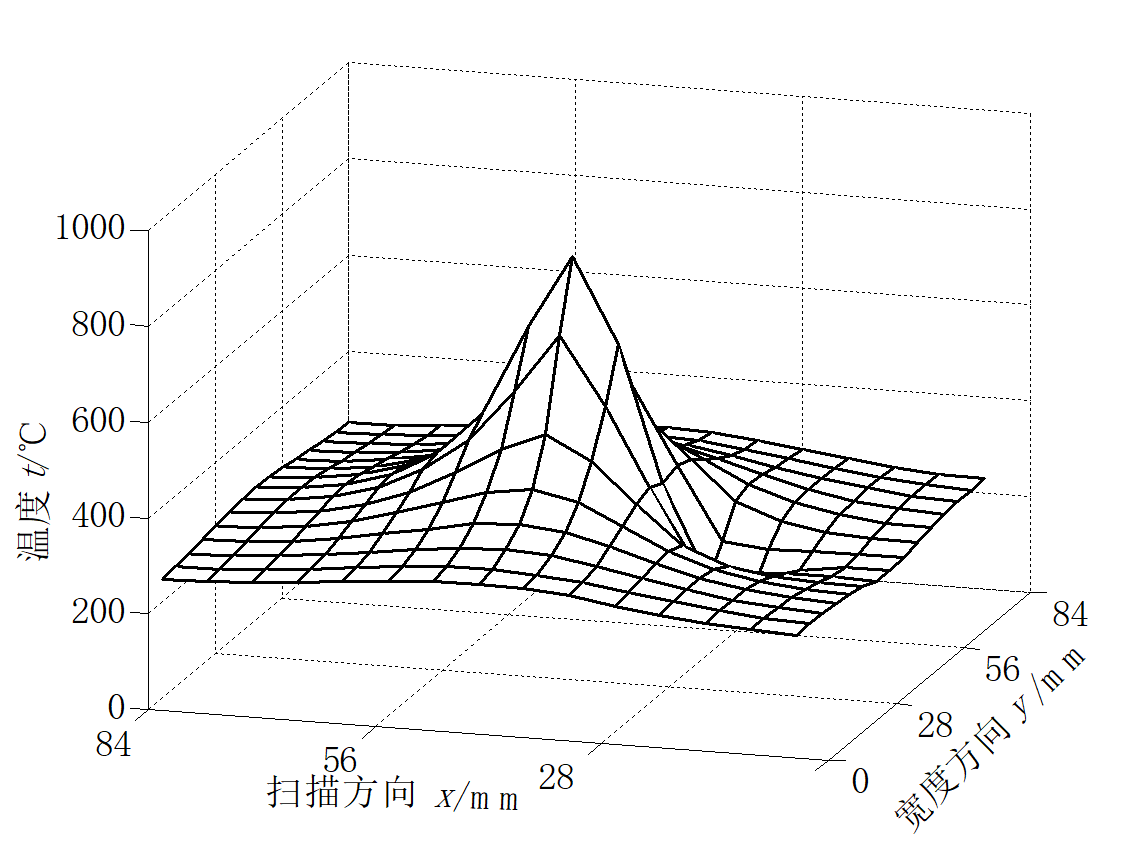
\includegraphics[width=0.4\textwidth]{fig21a.png}\label{fig1}}\hspace{30pt}
		\subfloat[图b标题]{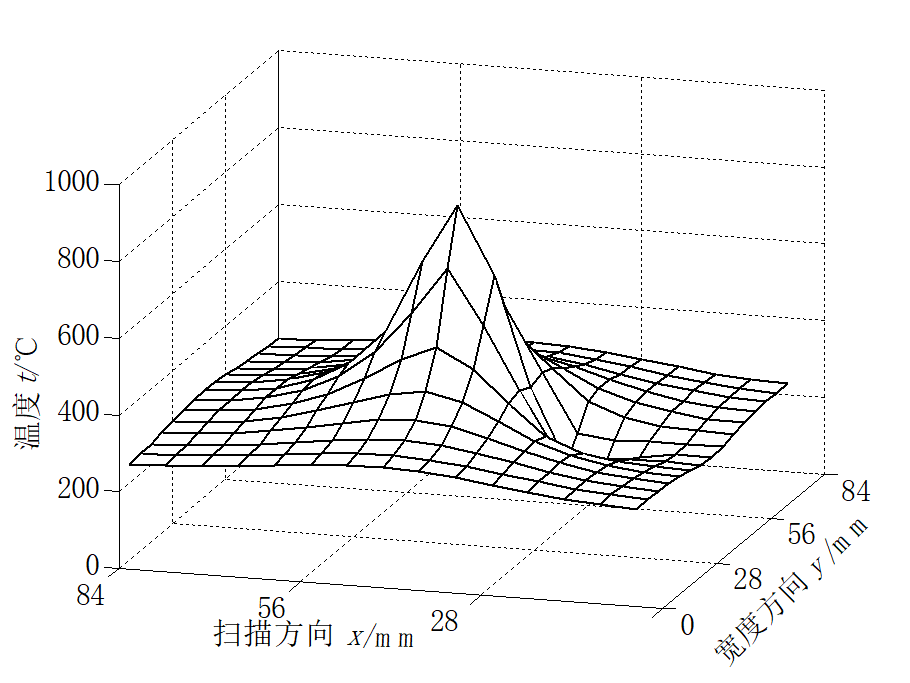
\includegraphics[width=0.4\textwidth]{fig21b.png}}
		\caption{跟随冷源对温度场的影响}
	\end{figure}
	
	\subsection{表格式要求}
	
	表中参数应标明量和单位的符号。表中字体及大小根据实际情况自行调整。行间距为单倍行距。表序号及表名称置于表的上方。
	
	表名称:正文中的表要有中文名称,表的中文名称为5号宋体字,不加粗,居中并位于表上;
	
	表尺寸:表尽量以一页的页面为限,一旦超限要加续表;
	
	表位置:表居中排列;
	
	表格式:三线表。三线表的组成要素包括:表序、表题、项目栏、表体、表注。三线表通常只有3条线,即顶线、底线和栏目线。其中顶线和底线为粗线,栏目线为细线。如下表:
	
	\begin{table}[!ht]
		\caption{标题内容}\label{tab:lable}
		\begin{tabular*}{\hsize}{@{}@{\extracolsep{\fill}}lllllllllllll@{}}
			\toprule
			$p_{t}$  &21  &22  &20  &15  &10  &8   &5   &10  &18  &10  &14  &18\\
			\midrule
			$c_{t}$  &5   &13  &10  &10  &10  &10  &10  &10  &10  &10  &10  &10\\
			$h_{t}$  &10  &5   &5   &5   &5   &5   &5   &5   &5   &5   &5   &5 \\
			$s_{t}$  &100 &100 &100 &100 &100 &100 &100 &100 &100 &100 &100 &100\\
			$d_{t}$  &30  &45  &50  &55  &45  &55  &90  &80  &90  &65  &80  &70 \\
			\bottomrule
		\end{tabular*}
	\end{table}
	
	\subsection{公式}
	
	公式:编号用括号括起写在右边行末,其间不加虚线。
	
	公式序号:分章编号,如(3-1)、(3-2)、...。对其中字母代表意义的解释紧随其后并顶格书写。公式中的字符应调整到小四号字左右。公式采用公式编辑器编写。如下公式:
	
	\begin{equation}
		x=\frac{b+\sqrt{c+d}}{b-\sqrt{c-d}}
	\end{equation}
	其中,b,c,d分别为矫正系数
	
	公式位置:公式居中,公式上下分别要与正文间隔一空行,公式序号在公式所在行的最右边列出。一行写不完的长公式,最好在等号或运算符等数学符号前换行。
	
	将分数的分子分母平列在一行而用斜线分开时,应注意避免含义不清的情况,例如,$a\slash bcosx$会有(a/b)cosx和a/(bcosx)两种理解。公式中分数线的长短要写清楚,主要分数线要与等号对齐。

	这是一条引用\cite{alahiSocialLSTMHuman2016}。
	
	{\centering\chapter{规范表达注意事项}}
	{\centering\chapter{装订注意事项}}
	{\centering\chapter{结论}}
	
	% -----------使用bib文件储存参考文献信息------------
	{\centering \bibliography{reference.bib}}
	\addcontentsline{toc}{chapter}{参考文献}%将“参考文献加入目录中”
	\bibliographystyle{gbt7714-2005-numerical}

	
	\thispagestyle{plain}
	
	
%	------------致谢-------------
	{\centering \chapter *{致\qquad 谢}}
	
	\addcontentsline{toc}{chapter}{致\qquad 谢}%将“参考文献加入目录中”
	\markboth{}{}
	感谢感谢感谢

\end{document}